El primer prototip del detector de triti desenvolupat en la col·laboració TRITIUM s'anomena TRITIUM-IFIC-0, el qual va ser dissenyat i construït als tallers de l'IFIC, a València. Aquest va consistir en un prototip a escala que pretenia ser una prova de concepte, és a dir, es pretenia provar la viabilitat de la tecnologia proposada per la col·laboració TRITIUM (fibres centellejadores llegides per fotosensors) per a la detecció de baixes activitats de triti al aigua.

Aquest prototip consisteix en un conjunt de $35$ fibres centellejadores, mostrades a la Figura \ref{subfig:FibresDobladesTritiumIFIC0}, cadascuna de les quals té $1~\mm$ de diàmetre i $20~\cm$ de longitud. Aquestes van ser polides manualment i es van unir amb una pesa metàl·lica als extrems la qual s'utilitzada per fixar-les en el atuell del prototip. Aquest atuell, mostrat a la Figura \ref{subfig:PrototipTritiumIFIC0}, consisteix en una estructura de PVC. La forma corbada d'aquest li confereix una major radioseguretat al preu d'una menor eficiència en la detecció del triti, un preu a pagar en els primers prototips ja que simplement es pretenia realitzar una prova de concepte i no un disseny final optimitzat. Dos PMTs calibrats, model R$8520-460$ de Hamamatsu Photonics \cite{DataSheetPMTs}, van ser ensamblats a aquestes fibres utilitzant greix òptic \cite{OpticalGrease} i llegits en coincidència temporal.

\begin{figure}
\centering
    \begin{subfigure}[b]{0.5\textwidth}
    \centering
    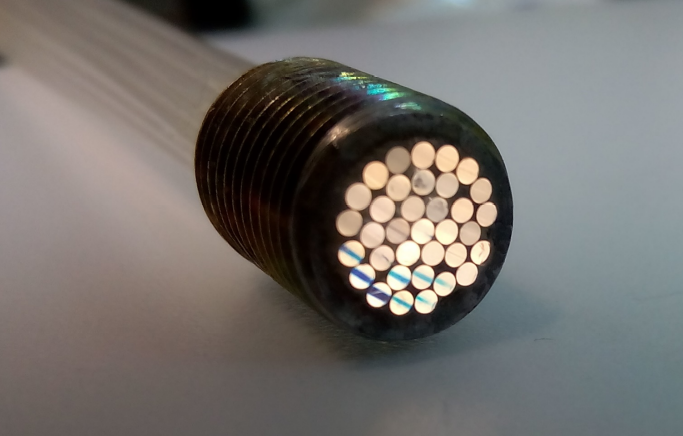
\includegraphics[width=\textwidth]{12Summary/5Prototypes/52PreliminarPrototypes/521TritiumIFIC0/Metalic_piece_of_fiber_bundle.png}  
    \caption{\label{subfig:PesaMetalicaFibresTritiumIFIC0}}
    \end{subfigure}
    \hfill
    \begin{subfigure}[b]{0.4\textwidth}
    \centering
    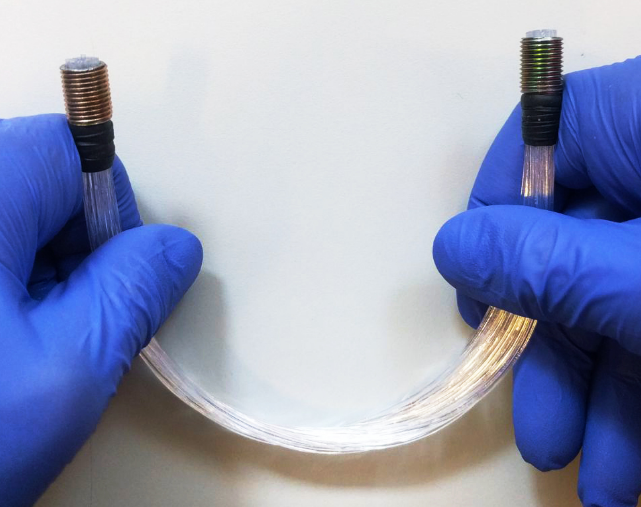
\includegraphics[width=\textwidth]{12Summary/5Prototypes/52PreliminarPrototypes/521TritiumIFIC0/FiberBundleBent.png}  
    \caption{\label{subfig:FibresDobladesTritiumIFIC0}}
    \end{subfigure}
    \hfill
    \begin{subfigure}[b]{0.7\textwidth}
    \centering
    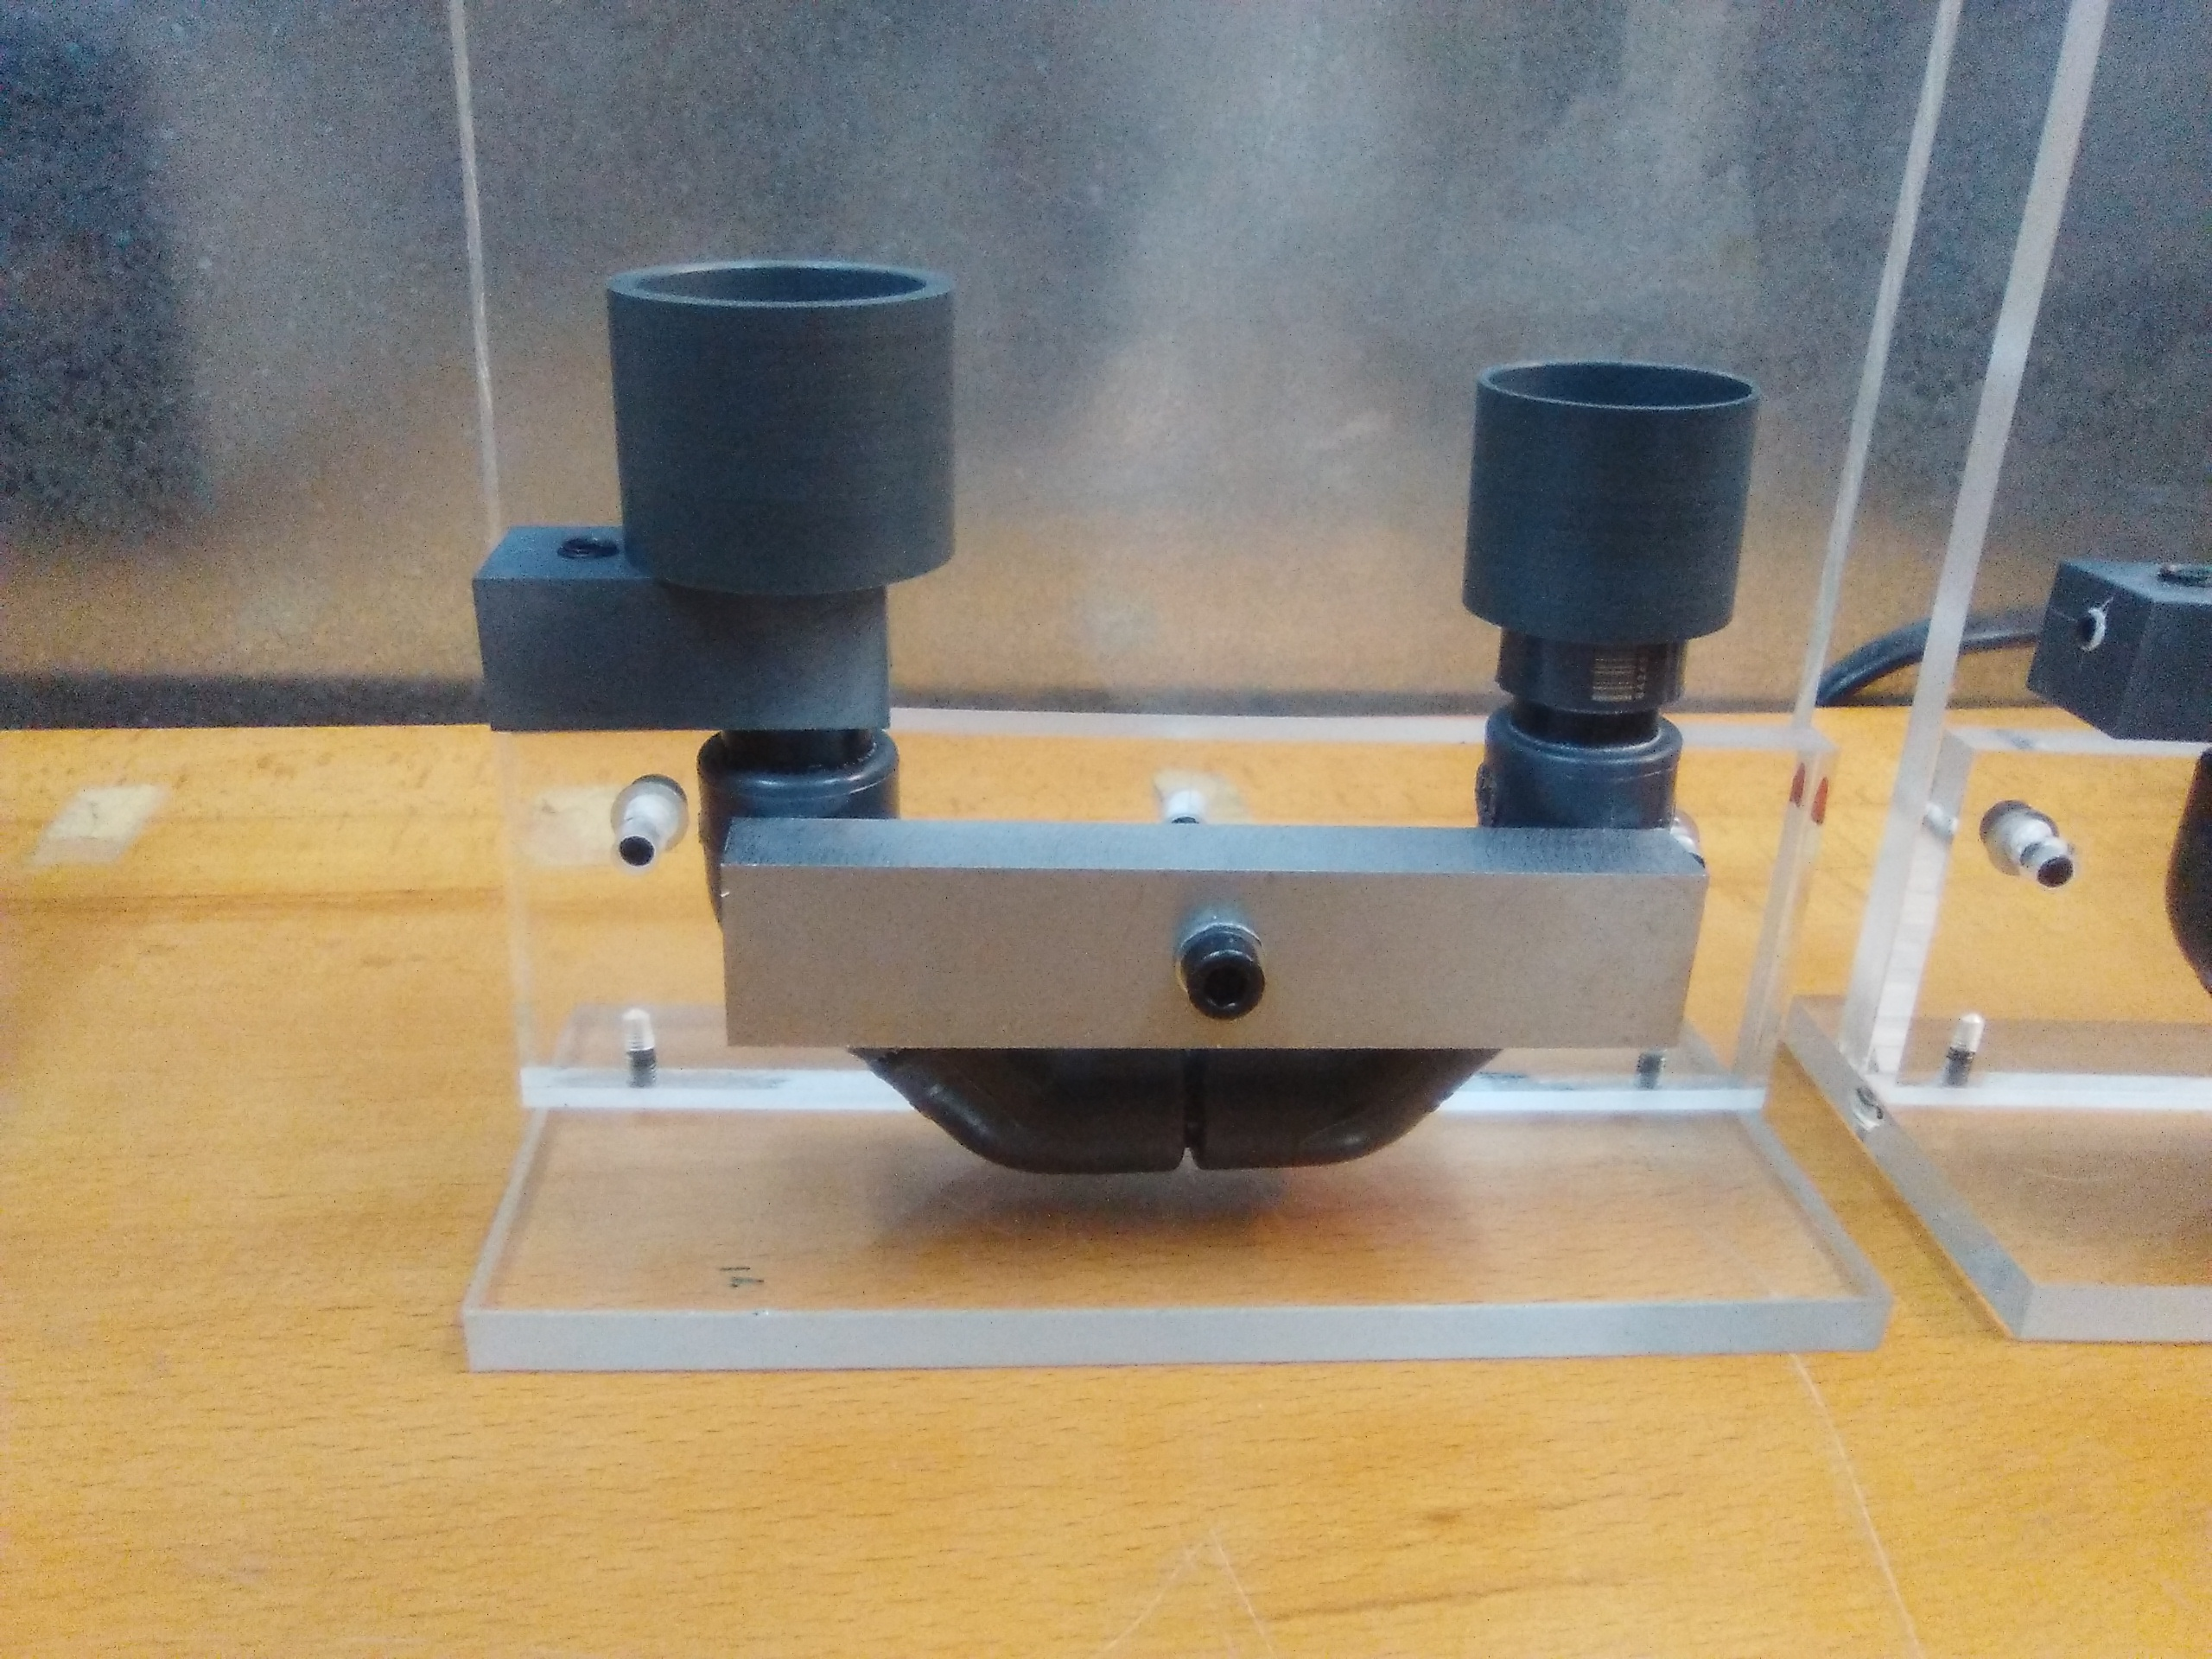
\includegraphics[width=\textwidth]{12Summary/5Prototypes/52PreliminarPrototypes/521TritiumIFIC0/Tritium_IFIC_0.jpg}  
    \caption{\label{subfig:PrototipTritiumIFIC0}}
    \end{subfigure}
 \caption{a) Pesa metàl·lica utilitzada per unir les fibres centellejadores del prototip TRITIUM-IFIC-0. b) Fibres centellejadores utilitzades en el prototip TRITIUM-IFIC-0. c) Prototip TRITIUM-IFIC-0.} \label{fig:TritiumIFIC0s}
\end{figure}

Com ja hem comentat a la secció \ref{subsec:SistemaRebuigFons}, el detector presenta una taxa de recompte no nul·la en absència de font radioactiva a causa de l'existència del fons radioactiu (elements radioactius presents a l'entorn o rajos còsmics procedents de fonts extraterrestres). Aquesta radioactivitat mesurada pel detector ha de ser quantificada i sostreta de la mesura amb font radioactiva per determinar l'activitat de la font emprada (aigua tritada en el nostre cas). Per realitzar aquesta tasca es van construir dos prototips idèntics, un omplit únicament amb aigua hiperpura, que ens referirem com el prototip del fons i servirà per determinar aquest fons radioactiu, i un altre omplit amb una dissolució d'aigua tritiada d'activitat específica coneguda ($\text{A}=99.696~\kilo\becquerel/\liter$), al que ens referirem com el prototip del senyal. L'activitat del triti mesurada per el prototip es obtinguda com la diferència de la mesura dels dos prototips.

Apenes es van mesurar esdeveniments utilitzant la coincidència temporal dels dos PMTs, probablement degut, entre altres coses, al disseny corbat del atuell, per tant es va realitzar la mesura individual dels PMTs. L'espectre d'energia mesurat al prototip del senyal, el prototip del fons i la diferència (espectre d'energia del triti) es mostren a la Figura \ref{fig:EspectresEnergeticsTritiumIFIC0}. Els contes per segon mesurats per a les tres situacions, obtinguts com la integral dels respectius espectres d'energia, són mostrats a la Tabla \ref{tab:ContesPerSegonTRITIUMIFIC0}. 

\begin{figure}
\centering
    \begin{subfigure}[b]{1\textwidth}
    \centering
    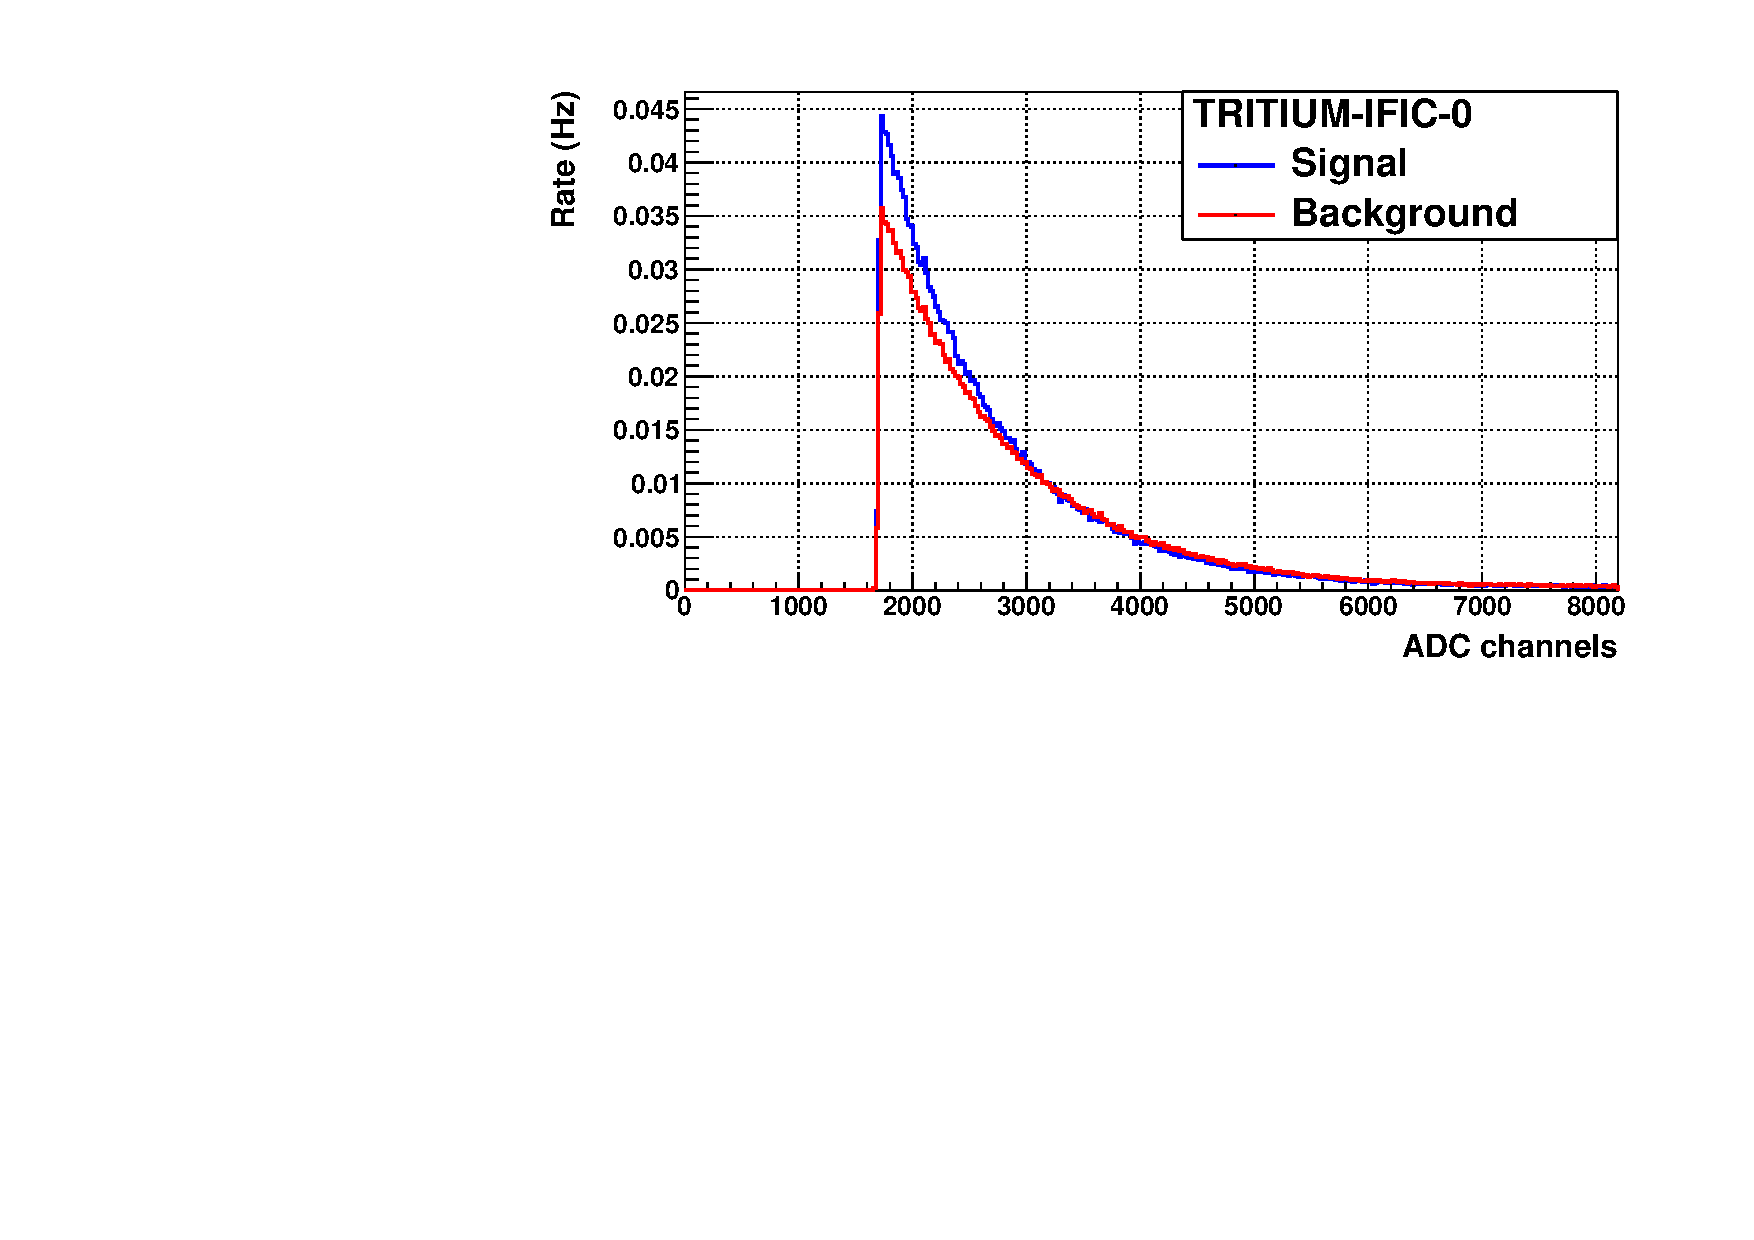
\includegraphics[width=\textwidth]{12Summary/5Prototypes/52PreliminarPrototypes/521TritiumIFIC0/TritiumIFIC0Signals.pdf}  
    \caption{.\label{subfig:EspectreSenyalFonsTritiumIFIC0}}
    \end{subfigure}
    \hfill
    \begin{subfigure}[b]{1\textwidth}
    \centering
    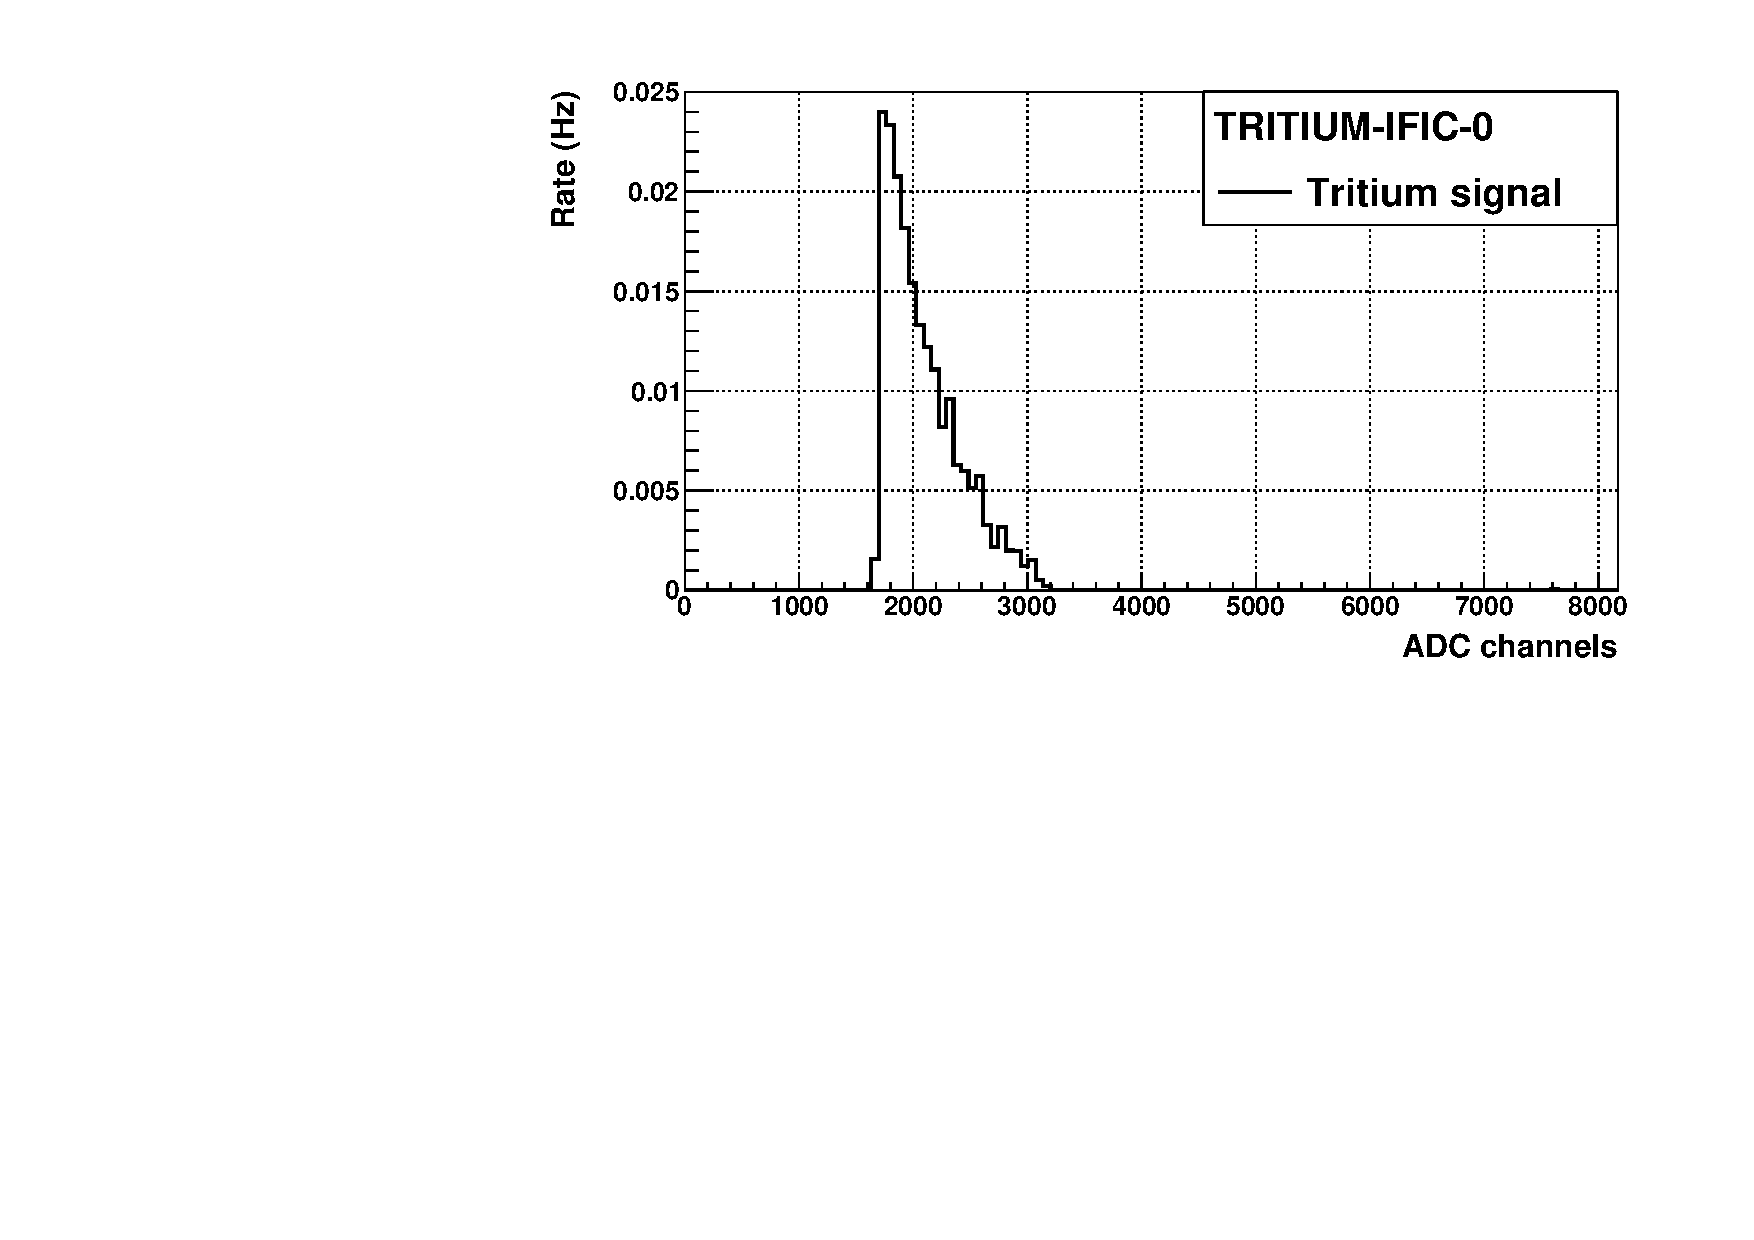
\includegraphics[width=\textwidth]{12Summary/5Prototypes/52PreliminarPrototypes/521TritiumIFIC0/TritiumIFIC0ClearRebin.pdf}  
    \caption{\label{subfig:EspectreTritiTritiumIFIC0}}
    \end{subfigure}
 \caption{Espectres d'energia mesurats amb el prototip TRITIUM-IFIC-0. a) Espectres mesurats amb els prototips de senyal i fons. b) Espectre del triti.}
 \label{fig:EspectresEnergeticsTritiumIFIC0}
\end{figure}

\begin{table}[htbp]
\centering{}%
\begin{tabular}{cc}
\toprule 
Espectres & Contes/segón \tabularnewline
\midrule
\midrule 
Prototip del senyal & $2.27 \pm 0.06$ \tabularnewline
Prototip del fons & $2.06 \pm 0.06$ \tabularnewline  
Espectre de triti & $0.21 \pm 0.085$ \tabularnewline
\bottomrule
\end{tabular}
\caption{Contes per segon mesurats amb el prototip TRITIUM-IFIC-0.}
\label{tab:ContesPerSegonTRITIUMIFIC0}
\end{table}

Tenint en compte l'activitat inicial coneguda i l'àrea activa del detector, s'obté una eficiència específica en la detecció del triti de
$$S = (9.59 \pm 3.88)\cdot{} 10^{-6}~\frac{cps}{\kilo\becquerel/\liter \cdot{} \cm^{2}}$$
eficiència similar a algunes de les obtingudes en detectors de triti desenvolupats en altres col·laboracions \cite{Muramatsu, Moghissi}.

Es van trobar alguns problemes que van ser resolts en el disseny del següent prototip, TRITIUM-IFIC-1:

\begin{enumerate}
\item{} Es va comprovar amb un test de laboratori que la curvatura de les fibres produïa una pèrdua exesiva de fotons ja que aquest necessitaven fer més reflexions fins a arribar als fotosensors. Aquest problema es va resoldre simplement dissenyant un atuell per al prototip TRITIUM-IFIC-1 on les fibres estigueren rectes.

\item{} A més es va aplicar un protocol de neteja sobre les superfícies de les fibres utilitzades al prototip TRITIUM-IFIC-1. Amb aquest s'aconsegueix incrementar l'eficiència de col·lecció dels fotons al voltant d'un $30\%$.

\item{} També es va observar que els fotons que havien escapat de les fibres eren ràpidament absorbits pel atuell de PVC i, per tant, perduts. Un material més adequat per a aquest seria, per exemple, el politetrafluoroetilè (PTFE), que presenta un factor de reflexió dels fotons visibles d'aproximadament el $95\%$, augmentant la probabilitat que el fotó pugui ser detectat pels fotosensors.

\item{} Finalment, s'utilitza una estructura per mantenir una distància de $1~\cm$ entre fibres. Aquesta modificació va ser utilitzada per assegurar que l'aigua tritiada cobris tota la superfície activa del detector.

\end{enumerate}

Tenint en compte tots aquests problemes identificats en el disseny del primer prototip, es va dissenyar i construir als tallers de l'IFIC un segon prototip, anomenat TRITIUM-IFIC-1, mostra a la Figura \ref{fig:TritumIFIC1s}, on totes les solucions proposades foren implementades .

\begin{figure}[h]
\centering
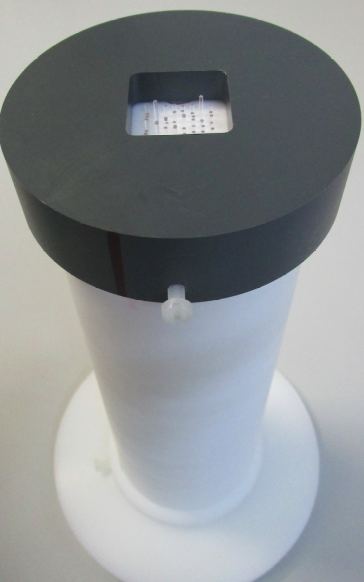
\includegraphics[scale=0.4]{12Summary/5Prototypes/52PreliminarPrototypes/522TritiumIFIC1/TritiumIFIC1a.png}
\caption{Vista general del prototip TRITIUM-IFIC-1.\label{fig:TritumIFIC1s}}
\end{figure}

El prototip TRITIUM-IFIC-1 consisteix en 64 fibres de $1~\mm$ de diàmetre i $20~\cm$ de longitud polides manualment i organitzades en una matriu de $8\times 8$ de PTFE, mostrada a la Figura \ref{fig:EstructuraPTFEFibresTritiumIFIC1}. Aquesta matriu està situada a l'interior d'un atuell de PTFE i llegides per un PMT calibrat model R$8520-460$ de Hamamatsu Photonics \cite{DataSheetPMTs} ensamblat amb greix òptic \cite{OpticalGrease}.

\begin{figure}[h]
\centering
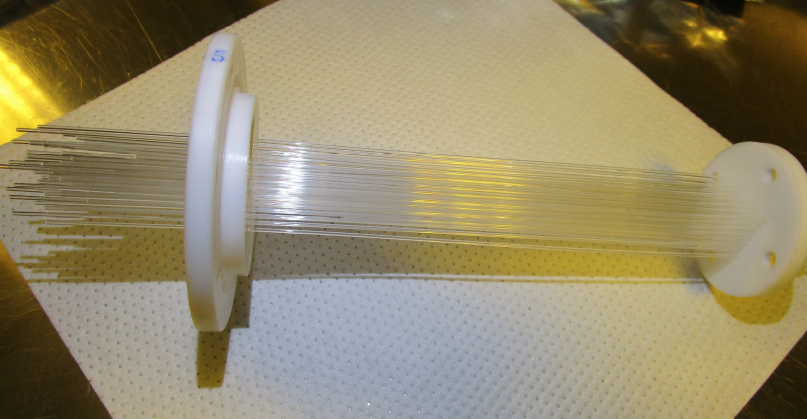
\includegraphics[scale=0.4]{12Summary/5Prototypes/52PreliminarPrototypes/522TritiumIFIC1/FiberMatrixTeflonStructure.png}
\caption{Estructura de PTFE utilitzada al prototip TRITIUM-IFIC-1.\label{fig:EstructuraPTFEFibresTritiumIFIC1}}
\end{figure}

Es van mesurar espectres d'energia similars al cas del prototip anterior, els quals es mostren a la Figura \ref{fig:EspectresEnergeticsTRITIUMIFIC1}. L'activitat de la dissolució de triti utilitzada va ser la mateixa que la utilitzada en l'experiència anterior. Els contes per segon mesurats pel prototip TRITIUM-IFIC-1 són mostrats a la Taula \ref{tab:ContesPerSegonTRITIUMIFIC1}

\begin{figure}
\centering
    \begin{subfigure}[b]{1\textwidth}
    \centering
    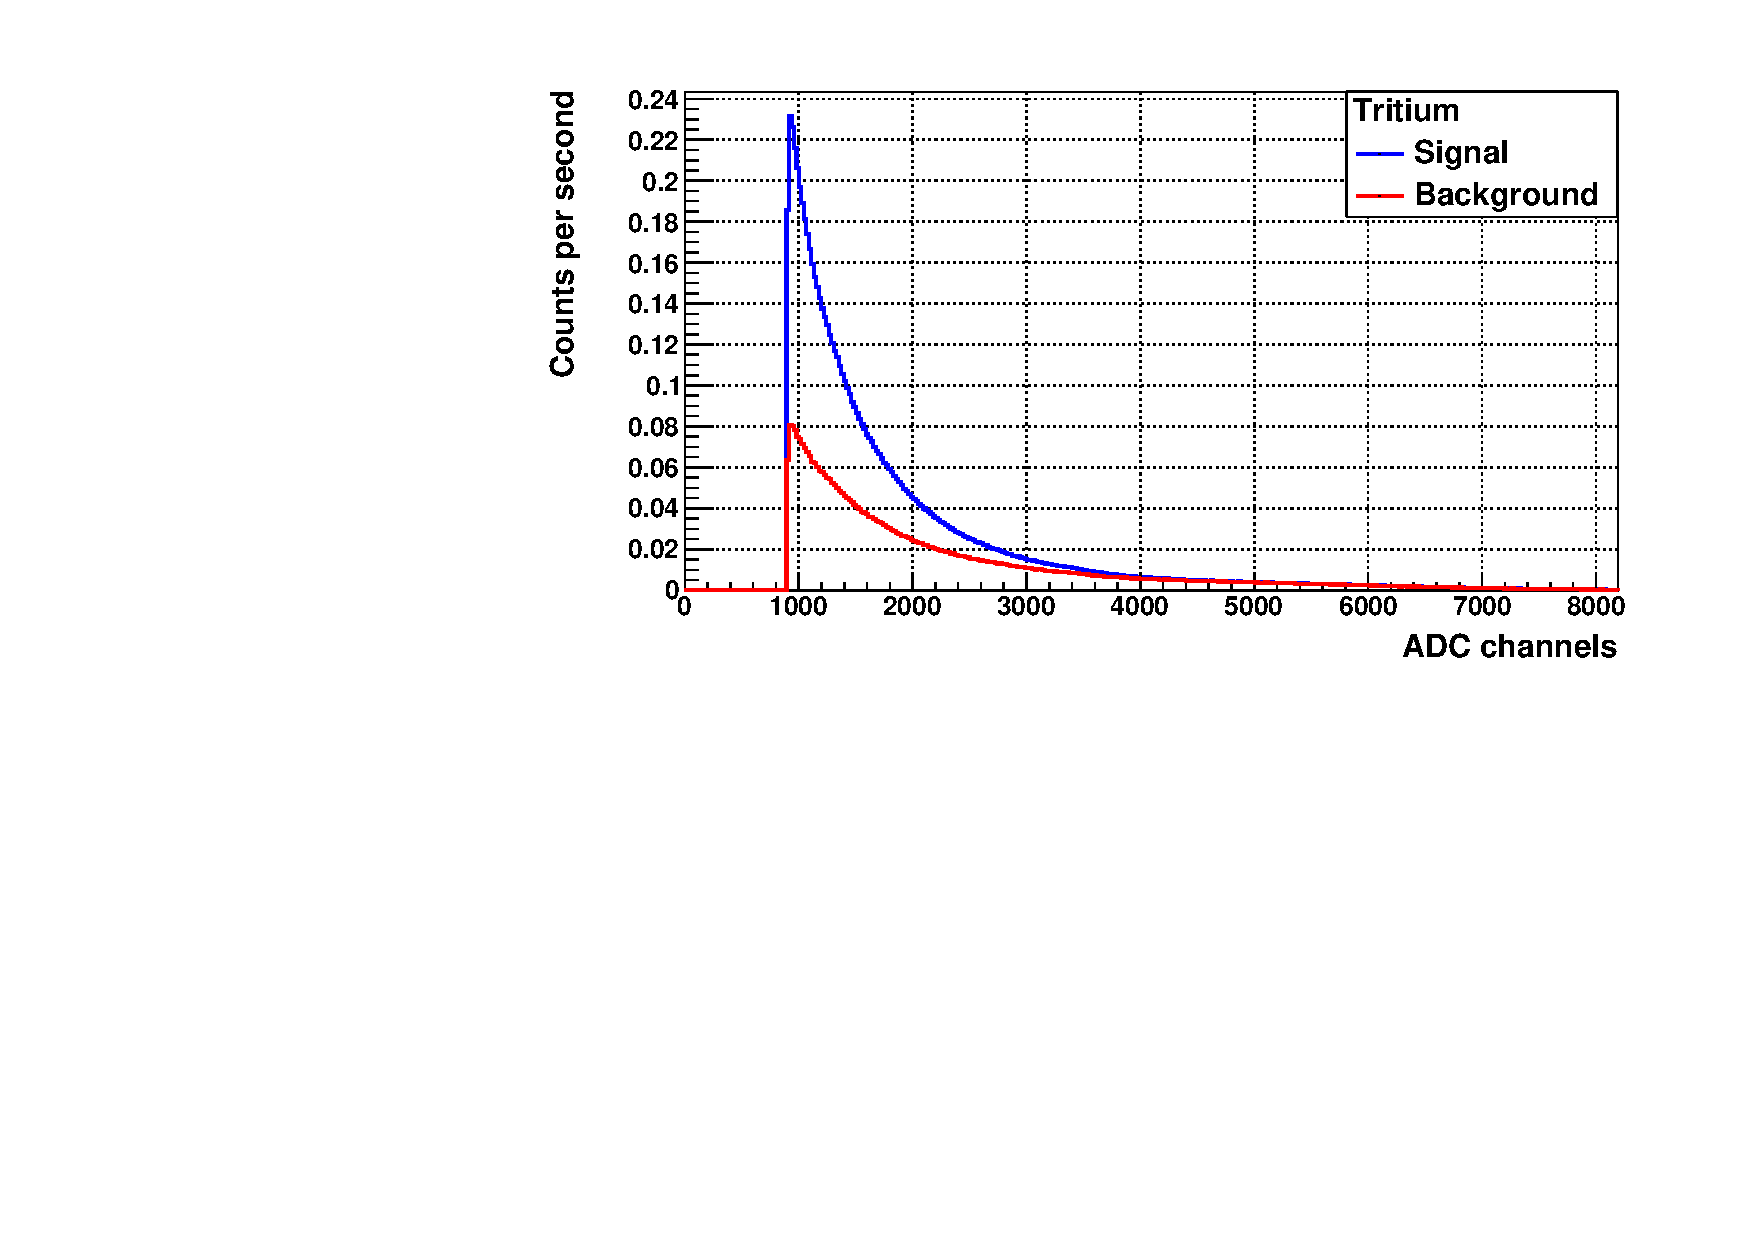
\includegraphics[width=\textwidth]{12Summary/5Prototypes/52PreliminarPrototypes/522TritiumIFIC1/TritiumIFIC1Signals.pdf}  
    \caption{\label{subfig:EspectreEnergeticSenyalFonsTritiumIFIC1}}
    \end{subfigure}
    \hfill
    \begin{subfigure}[b]{1\textwidth}
    \centering
    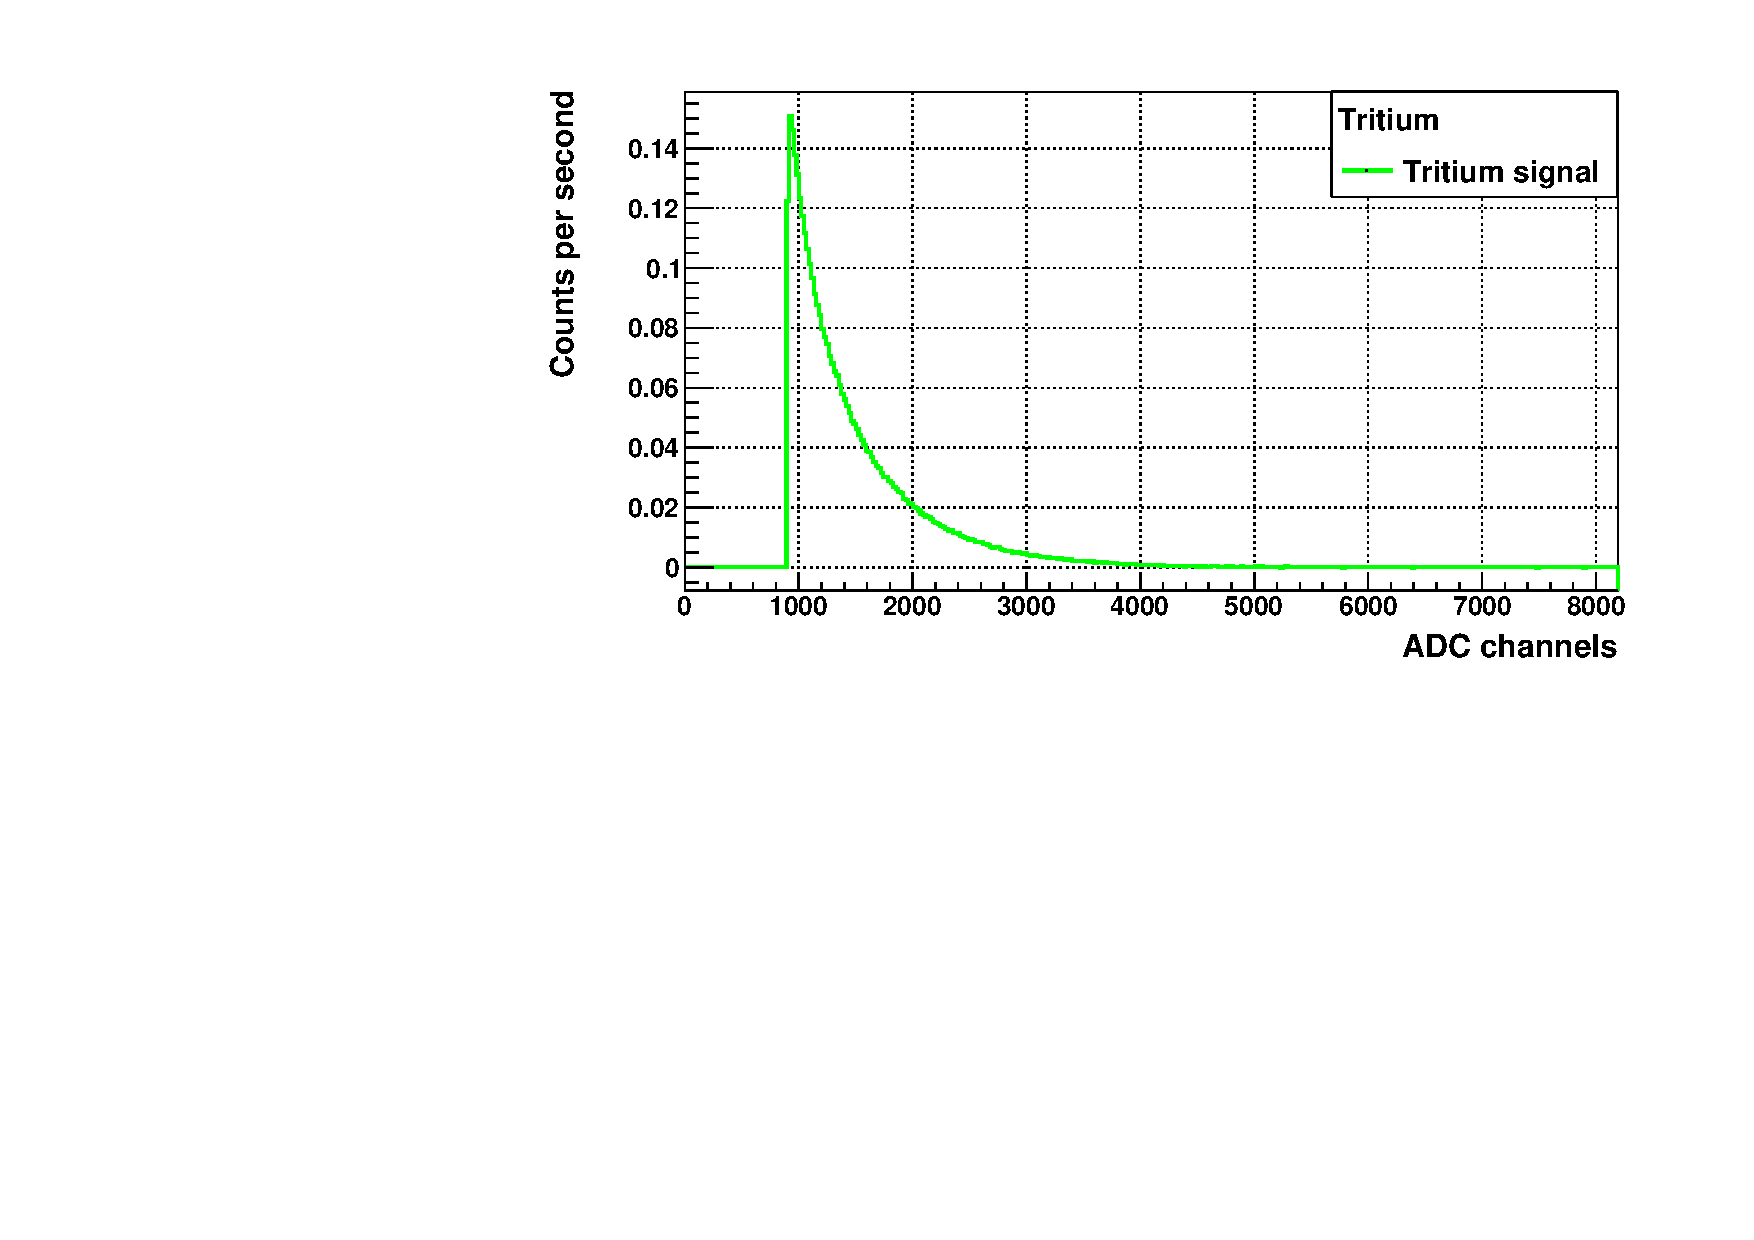
\includegraphics[width=\textwidth]{12Summary/5Prototypes/52PreliminarPrototypes/522TritiumIFIC1/TritiumIFIC1Clear.pdf}  
    \caption{\label{subfig:EspectreEnergeticTritiTritiumIFIC1}}
    \end{subfigure}
 \caption{Espectres d'energia mesurats amb el prototip TRITIUM-IFIC-1. a) Espectre d'energia de senyal i fons. b) Espectre d'energia del triti.}
 \label{fig:EspectresEnergeticsTRITIUMIFIC1}
\end{figure}

\begin{table}[htbp]
\centering{}%
\begin{tabular}{cc}
\toprule 
Espectres & Contes/segón  \tabularnewline
\midrule
\midrule 
Prototip del senyal & $7.82 \pm 0.11$ \tabularnewline
Prototip del fons & $3.99 \pm 0.08$ \tabularnewline  
Espectre de triti & $3.83 \pm 0.13$ \tabularnewline
\bottomrule
\end{tabular}
\caption{Contes per segon mesurats amb el prototip TRITIUM-IFIC-1.}
\label{tab:ContesPerSegonTRITIUMIFIC1}
\end{table}

L'eficiència específica en la detecció del triti obtinguda per a aquest detector es de
$$S = (9.56 \pm 0.40)\cdot{} 10^{-5}~\frac{cps}{\kilo\becquerel/\liter \cdot{} \cm^{2}}$$
un ordre de magnitud millor que l'obtinguda amb el prototip anterior. Aquest ordre de magnitud es deu al conjunt de totes les modificacions realitzades en aquest disseny. Aquesta eficiència específica obtinguda és similar a la millor eficiència específica obtinguda fins ara amb detectors de triti similars desenvolupats en altres col·laboracions \cite{Hofstetter1, Hofstetter2}. Veiem per tant que el detector de triti desenvolupat en la col·laboració TRITIUM és competitiu amb els detectors similars desenvolupats fins ara.